\chapter{The Equivalence Mapping}
\label{chap:equiv_mapping}

\section{Look-ahead and Searching-states}

Given that $T_1 \leq_k T_2$, is the mapping $\psi_k: x\mapsto x'$ finitely describable?

\begin{example}

Set $\Lambda=L[ab\cdot (cc)^\star\cdot (ab+ba)]$ and $k=2$, and let $T_1$ and $T_2$ be the transducers last drawn on the whiteboard (``wb6''), satisfying $T_1\leq_{k,\Lambda} T_2$ with the (infinite) equivalence mapping $\psi^\star: (\Sigma_I^k)^\star \rightarrow (\Sigma_I^k)^\star$.

We claim that for any $r$, there exists no (finitely describable) function $\psi: (\Sigma_I^{rk})^\star \rightarrow (\Sigma_I^{rk})^\star$ such that $\psi^\star(x)=\psi(x)$ for all input words $x$.

Indeed, let $r$ be given, and assume by contradiction that such $\psi$ exists. Now consider the input word $x=ab\cdot c^{rk-2}$. $\psi(x)$ must start with either $ab$ or $ba$. Without loss of generality, assume the former, and consider the input word $x':=x\cdot ba\cdot c^{rk-2}$. $\psi$ works on $r$ rounds each time, so that the first $r$ rounds are fixed when it reads the $(r+1)$-th round. Since $\psi(x')$ must induce a valid path in $T_2$, the only option for the $(r+1)$-th round of $\psi(x')$ is $ab$. Hence, the output of $T_1$ on $x'$ is different from the output of $T_2$ on $\psi(x')$, and we have a contradiction.

This example only works if we assume that $\psi$ is "ignorant" of the fact that, actually, we will \emph{never} want to shuffle the very first round to be $ba$. This is a piece of knowledge so simple that it is not reasonable to have it hidden from $\psi$.

(On the other hand, $\psi^\star$ must \emph{somehow} know how to shuffle the first round, albeit given the knowledge of the entire input...)

Nevertheless, let us try to get rid of $\Lambda$ and, afterward, try to work with a parametric round length $k$.

It worked! Find the generalized automata drawn on a piece of paper (``Dec 21$^\text{st}$''). \qedsymbol

\end{example}

The example shows that a "look-ahead" (actually, a "compound" of rounds or part-rounds) of $r$ rounds does not work, for any $r$. Also, it is clear that a "look-ahead" of a number not divisible by $k$ will not work either, since we must at least read the whole round to know the correct way to shuffle. Hence, this notion of "look-ahead" does not solve the problem.

What about the other notion of "look-ahead": a sliding-window variation of the former; that is, at any given round, we can see $r-1$ additional rounds in the future. It would not work either, with the same counter-example. Indeed, even if we know the future beforehand, it does not allow us to rewrite the past, so a mistake in the first round would not be fixed.

But how can we prevent such a mistake from happening? How would we have known, in this specific example, that the first round should be shuffled according to some future round, and know what that future round is, using just a finite number of states? Nothing bounds the number of rounds in-between, nor the number of rounds at the end or at the start. We will have to know that those rounds are "irrelevant"; that any shuffle would work. This sounds like a problem of state-isomorphism once more.

Actually, a finite-state machine is enough for the $\psi$ of the given example: The machine would read round-per-round, and once the round is of the form $a^{k-2}(ab+ba)$, it goes to a new state accordingly, and once the round is again of that form, it would decide the output for the first of them according to the second. Calculating the remainder of the output is simple.

We could find an \emph{ad-hoc} solution for our $\psi$, but does a solution always exist?

Firstly, let us generalize the way this latter $\psi$ was defined. We have a finite set of states that I will call "searching states", denoted $s_0, s_1, \dots, s_m$ (where $s_0$ also happens to be the initial state of the transducer); each of them is basically searching for a specific finite set of rounds, $F_0, \dots, F_m$. For any $i$, state $s_i$ would ignore all rounds of a form outside of $F_i$. State $s_m$ is the final state, and it ignores all rounds. When we say that a state ignores a round, we mean that it outputs any shuffle of that round. We want to remember which rounds were ``searched for and found.'' So the number of actual states is not $m$ but rather $1+\prod_{i=0}^m F_i$ (every non-initial state stores an $(m+1)$-tuple of rounds). Once we reach the last round, we look at the stored rounds and decide on the whole output (up to the last ``ignored'' rounds) accordingly. That is, the output is only decided upon reading the whole input; but it does so in a finite number of states. (What model is this?)

I claim that, had we dropped the word ``finite,'' this description would always hold true for $\psi$. Then, I further claim that this still holds true with the finiteness constraint.

Indeed, we can look at $\psi$ as an infinite-searching-state machine, where in every step it searches for any round (finite possibilities) and simply stores it inside itself. Upon reading the end of the input, it would output the correct shuffle for all rounds by heavy, finite calculations.

Now, let us suppose (hopefully by contradiction) that such a description, but finite, does not exist for $\psi$. So for any $m$, we need more than $m$ sets of rounds to ``search for,'' we could say. This means that there are at least $m$ distinct states, distant from $q_0$ by $k$-jumps, that act differently on different $k$-long rounds. In particular, there are at least $m$ distinct states. From here it easily follows that $m$ is upper-bounded by $n$, the number of states.

This gives the following lemma.

\begin{lemma}
Let $T_1\leq_k^\psi T_2$, then $\psi$ is finitely describable by a finite-searching-state machine of at most $n$ rounds.
\end{lemma}

\pagebreak

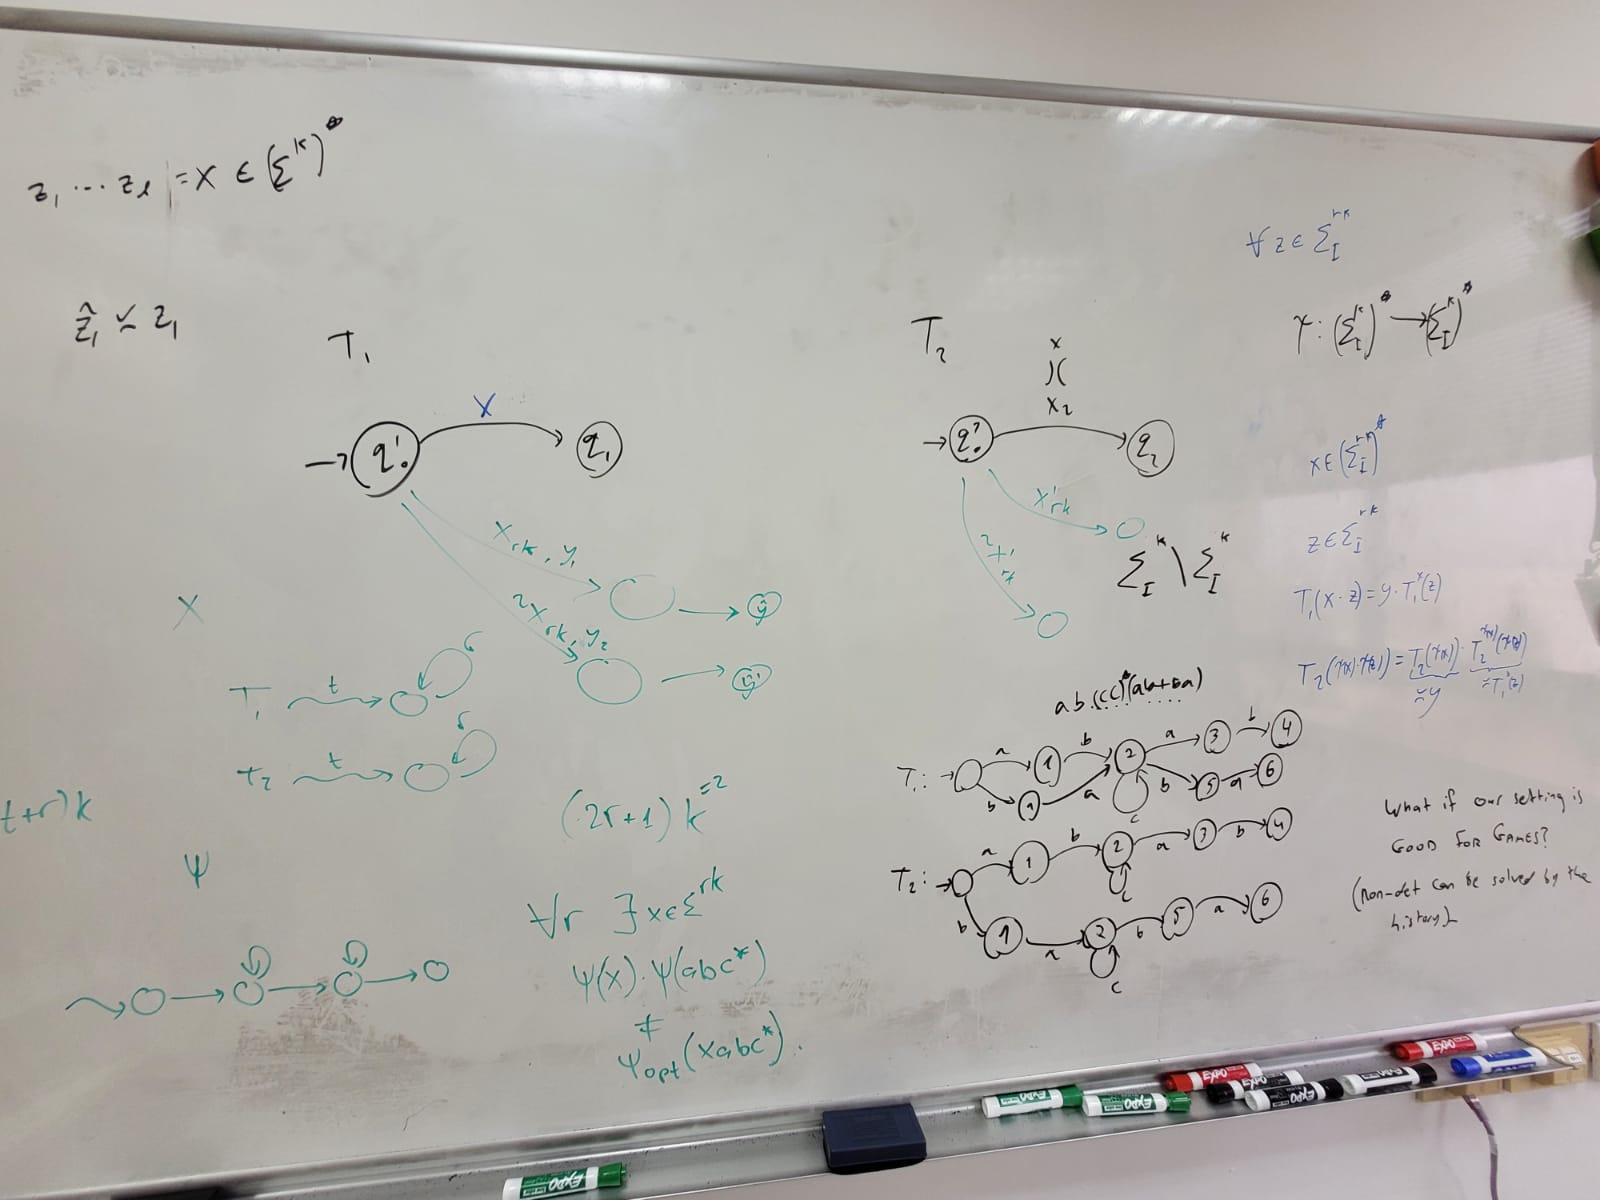
\includegraphics[width=\linewidth]{graphics/wb6.jpg}
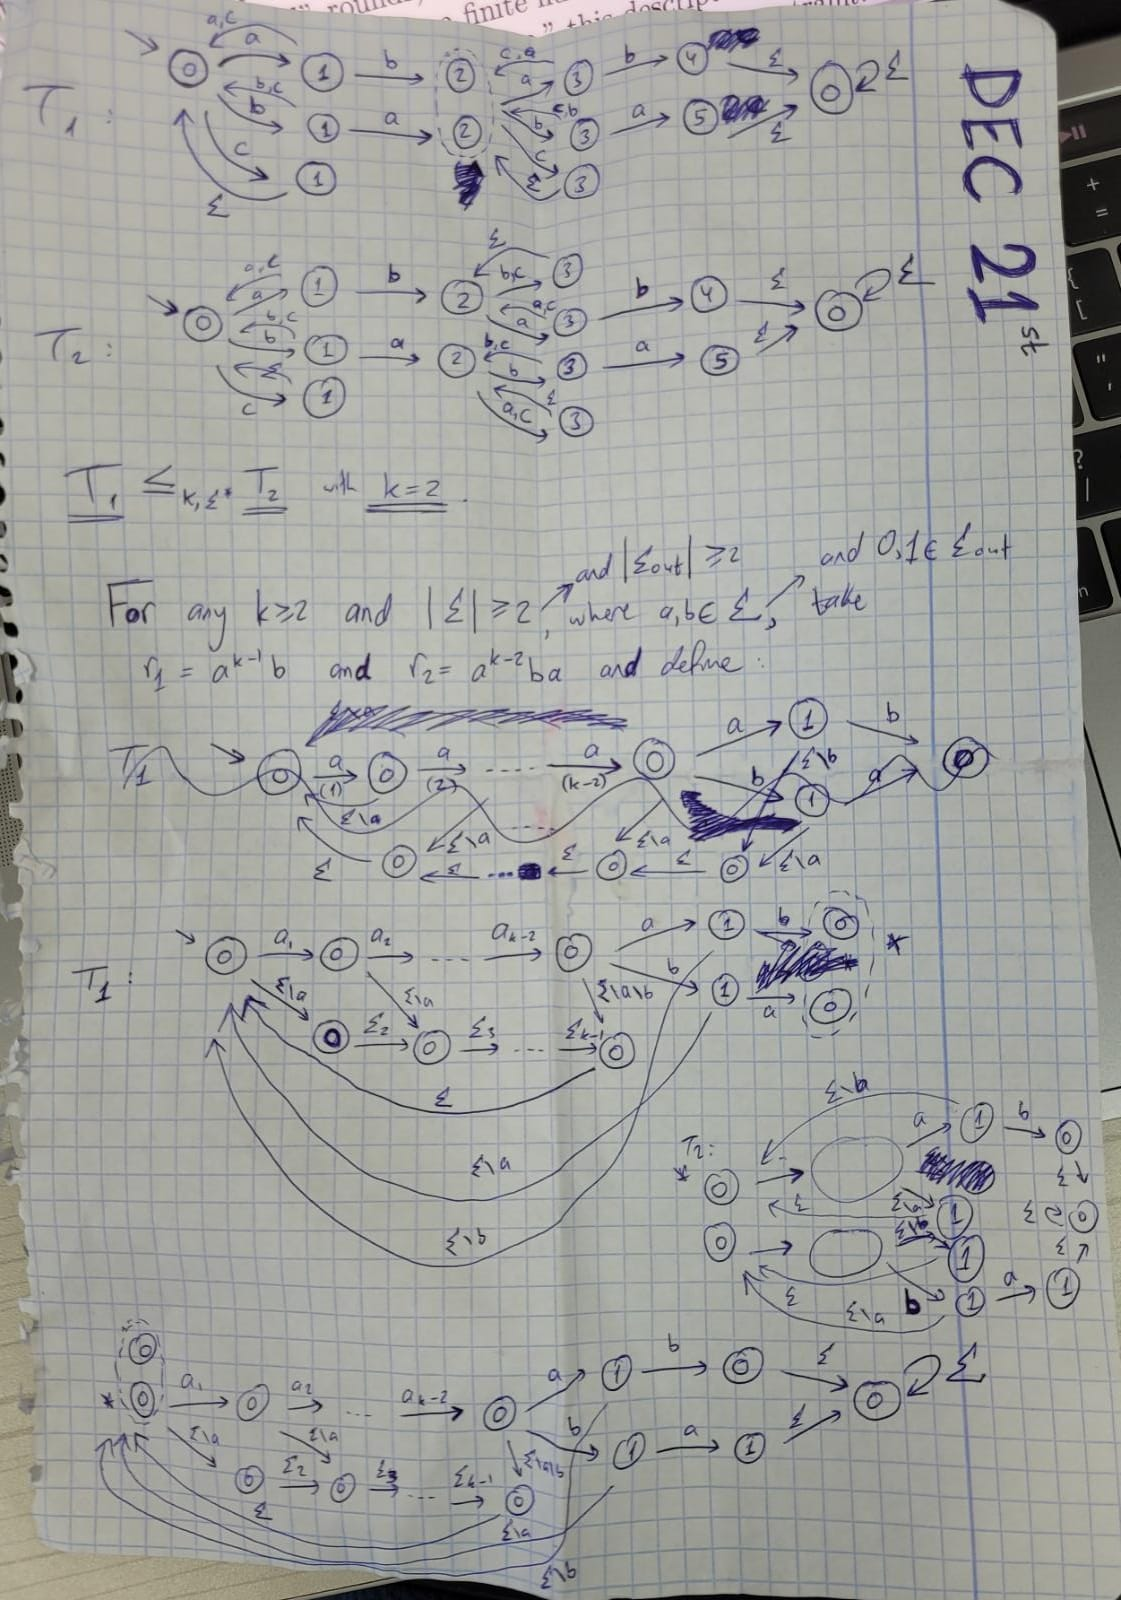
\includegraphics[width=\linewidth]{graphics/dec21.jpeg}